\documentclass{article}

% packages for math
\usepackage{amsthm}
\usepackage{amsmath}
\usepackage{amssymb}
\usepackage{amsfonts}

% package for including images
\usepackage{graphicx}

% TAKEN FROM OVERLEAF DOCUMENTATION
% https://www.overleaf.com/learn/latex/Code_listing
\usepackage{listings}
\lstset{language=Python}
\usepackage{xcolor}
\definecolor{codegreen}{rgb}{0,0.6,0}
\definecolor{codegray}{rgb}{0.5,0.5,0.5}
\definecolor{codepurple}{rgb}{0.58,0,0.82}
\definecolor{backcolour}{rgb}{0.95,0.95,0.92}
\lstdefinestyle{mystyle}{
  backgroundcolor=\color{backcolour},
  commentstyle=\color{codegreen},
  keywordstyle=\color{magenta},
  numberstyle=\tiny\color{codegray},
  stringstyle=\color{codepurple},
  basicstyle=\ttfamily\footnotesize,
  breakatwhitespace=false,
  breaklines=true,
  captionpos=b,
  keepspaces=true,
  numbers=left,
  numbersep=5pt,
  showspaces=false,
  showstringspaces=false,
  showtabs=false,
  tabsize=2
}
\lstset{style=mystyle}

% environment for solutions
\theoremstyle{remark}
\newtheorem*{solution}{Solution}

% capital letters for problem parts
\renewcommand{\theenumi}{\Alph{enumi}}

% no page numbers
\pagenumbering{gobble}

% UNCOMMENT IF YOU DON'T WANT PROBLEMS ON INDIVIDUAL PAGES
% \renewcommand{\pagebreak}{}

\newcommand{\vv}[1]{\mathbf{#1}}
\newcommand{\vspan}{\mathsf{span}}
\newcommand{\ran}{\mathsf{ran}}
\newcommand{\cod}{\mathsf{cod}}
\newcommand{\R}{\mathbb R}

\title{
  Homework 7
}
\author{CAS CS 132: Geometric Algorithms}
\date{Due: \textbf{Thursday November 2, 2023 at 11:59PM}}

\begin{document}
\maketitle

\subsection*{Submission Instructions}
\begin{itemize}
\item Make the answer in your solution to each problem abundantly clear (e.g., put a box around your answer or used a colored font if there is a lot of text which is not part of the answer).
\item Choose the correct pages corresponding to each problem in Gradescope. Note that Gradescope registers your submission as soon as you submit it, so you don't need to rush to choose corresponding pages.
  \textbf{For multipart questions, please make sure each part is accounted for.}
\end{itemize}
Graders have license to dock points if either of the above instructions are not properly followed.


\section*{Practice Problems}

The following list of problems comes from \textit{Linear Algebra and its Application 5th Ed} by David C.\ Lay, Steven R.\ Lay, and Judi J.\ McDonald.
They may be useful for solidifying your understanding of the material and for studying in general.
\textbf{They are optional, so please don't submit anything for them}.

\begin{itemize}
\item 2.5.1-3, 2.5.14, 2.5.26
\item Example 8 (useful for Problem 2), 2.7.2, 2.7.3-8, 2.7.12, 2.7.15, 2.7.16. 2.7.17
\end{itemize}


\pagebreak
\section{Sparse Factorizations}

In this problem, you will use the provided code in \texttt{sparse.py} to benchmark LU factorization and matrix inversion.

\begin{enumerate}
\item (2 points) The provided code includes a function \texttt{test\_matrix} which builds a matrix given a positive integer parameter. Write down the matrix returned by this function applied to 4.

\item (8 points) There is a function in the \texttt{scipy} library called \texttt{lu} which returns the LU factorization of a matrix.
  Use this to construct the LU factoration of $A = $ \texttt{test\_matrix(10 ** 3)}.
  This function returns a 3-tuple of matrices.
  The 2nd and 3rd entries are $L$ and $U$, respectively, where $A = LU$.

  Then use the function \texttt{np.linalg.inv} to construct the inverse $A^{-1}$ of this matrix.

  Finally, you can use the expression \texttt{len(np.nonzero(mat)[0])} to determine the number of nonzero entries in a 2D numpy array \texttt{mat}.
  \textbf{Write down the number of nonzero entires of $L$, $U$, and $A^{-1}$, where $A$ is the matrix \texttt{test\_matrix(10 ** 3)}, as well as the lines of code you used.}
\item (5 points)
  Uncomment the code at the end of the file \texttt{sparse.py} and run it.
  Write down the printed values and discuss what they mean.
  In particular, is the amount of time that it takes to factor versus invert consistent with our discussion in lecture?\footnote{You'll note that solving systems with the matrix inverse is faster than with the LU factorization. Even though the two have roughly the same theoretical guarantees, matrix-vector multiplication implementations tend to be better optimized.}
\end{enumerate}

\pagebreak

\begin{solution}
\end{solution}

\vfill

\pagebreak
\section{3D Graphics (Programming)}

\medskip

This week you will be building an interactive matplotlib widget which can manipulate 2D renderings of 3D wireframes.
Once you are done, it should look something like this, and you should be able to rotate and translate a wireframe object on screen using provided sliders.

\begin{center}
  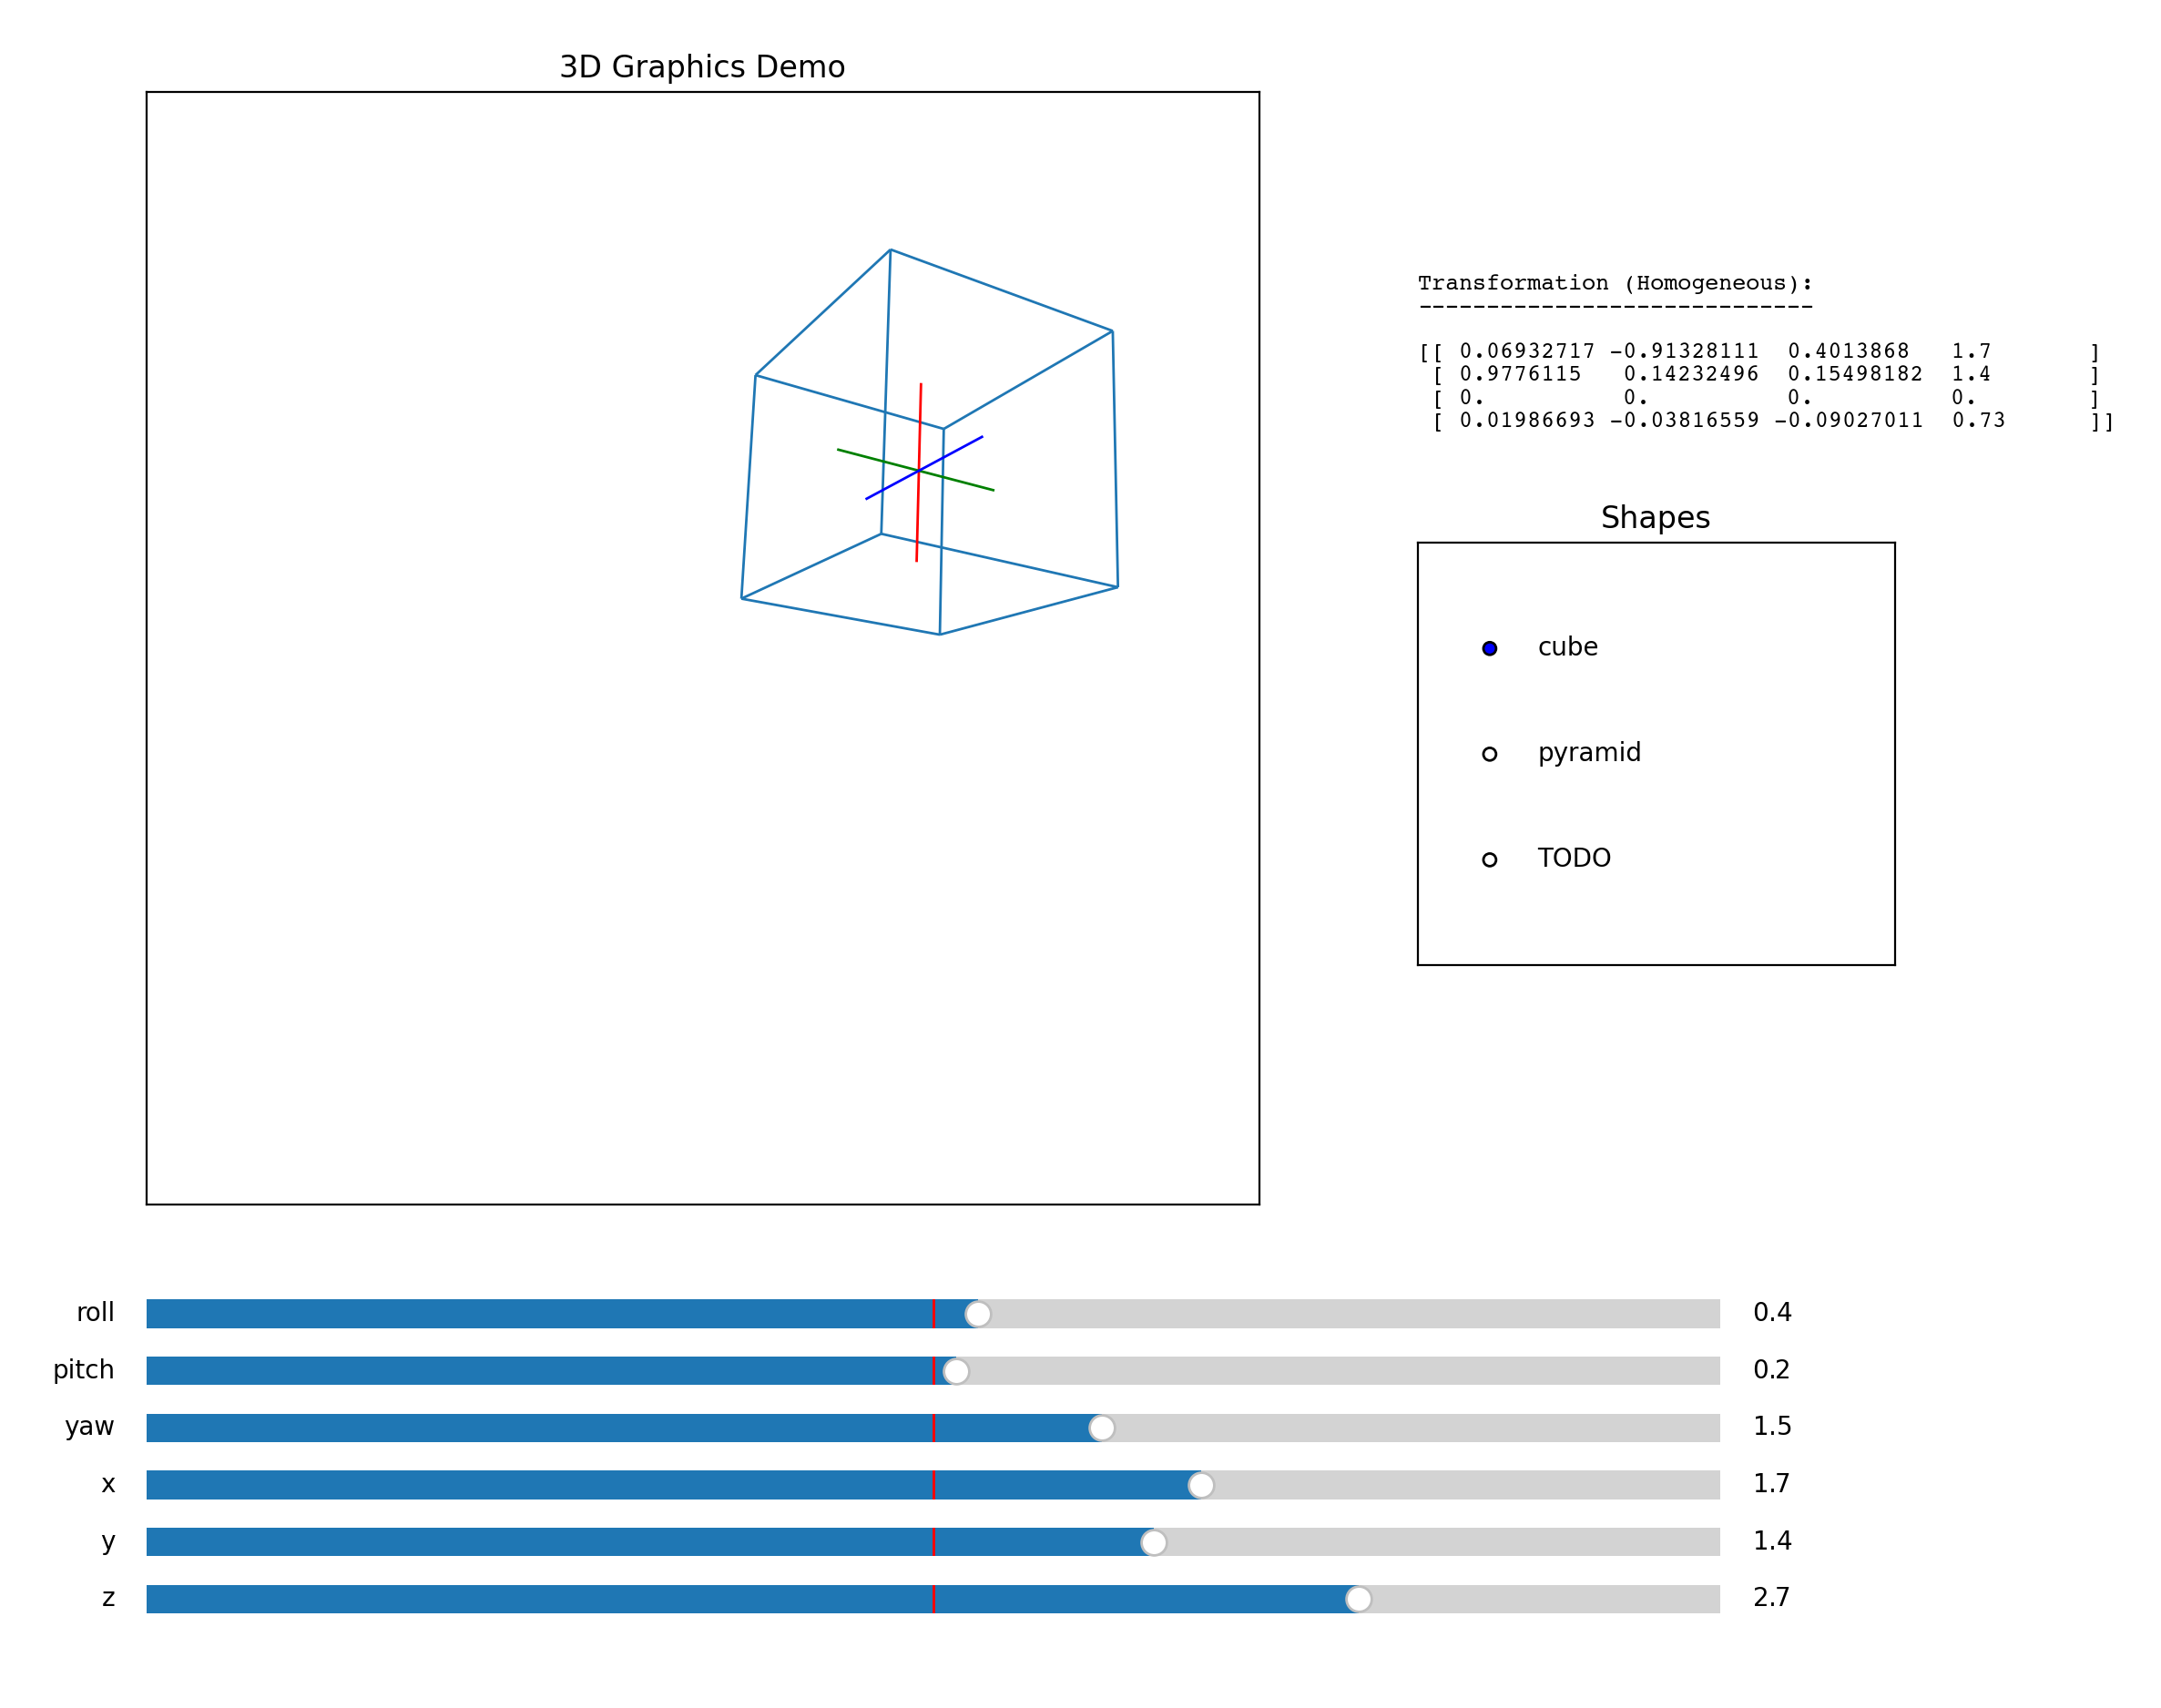
\includegraphics[scale=.25]{demo-screenshot.png}
\end{center}
You are given starter code in the file \texttt{hw07prog.py}.
\textbf{Don't change the name of this file when you submit.}
Also don't change the names of any functions included in the starter code.
\textbf{The only changes you should make are to fill in the provided TODO items.}
At a high level, the code works as follows.
\begin{itemize}
\item
  Wireframes are represented as lists of line segments, which are represented as 2-element lists of 3-tuples of floats (in other words, points in $\mathbb R^3$).
  You are provided with two simple wireframes, \texttt{cube} and \texttt{pyramid}.
  You will have an opportunity, for a small amount of extra credit, to build your own wireframe.
  You can use the structure of these two examples as a guide.
\item
  These wireframes are transformed into matrices whose columns are homogeneous coordinates of the endpoints of each segment in the wireframe.
  This is done by the function \texttt{shape\_to\_hom\_matrix}, which is implemented for you.
  At this point, red, green, and blue guide axes are included in the wireframe.
  So if the wireframe has 12 line segments, then this function returns a $4 \times (2 * (12 + 3)) = 4 \times 30$ matrix.
  In later steps we will call this matrix $W$.
  These matrices are collected in a dictionary called \texttt{shape\_matrices} which is used by the latter parts of the program.
  \textbf{You do not need to change any part of this code (that is, the code under the header ``SHAPES'')} except for potentially the extra credit wireframe.

\item
  The next step is to build the transformation that will ultimately augment the wireframe (in other words, the transform that will be applied to the matrix $W$).
  There are a number of basic matrix constructions you have to fill in:
  \begin{itemize}
  \item \texttt{perspective}
  \item \texttt{hom\_rotate\_x}
  \item \texttt{hom\_rotate\_y}
  \item \texttt{hom\_rotate\_z}
  \item \texttt{translate}
  \end{itemize}
  Once you fill in these functions, you will combine them into a single product of matrices which represent the transformation to the wireframe that will be rendered on screen.
  \textbf{You will implement this in the function \texttt{full\_transform\_matrix}.}
  Since this will be a multiplication, you are \textbf{required} to use the function \texttt{numpy.linalg.multi\_dot}.
  Please see the NumPy documentation for information on how to use this function.

  The matrix returned by this function should rotate and then translate the given wireframe, and then apply the perspective projection.
  It is important to remember that \textbf{the order of multiplications matters}.
  As a guide, when you finish, the roll axis should be red, and when you translate your shape, rotation should keep its center fixed.
  I will call the matrix returned by \texttt{full\_transform\_matrix} $T$ in latter steps.
\item
  The last step it to construct a collection of 2D line segments from the matrix $TW$.
  \textbf{You will be implementing this in \texttt{matrix\_to\_projection}.}
  Because of the perpsective projection which occurs in $T$, the columns of $TW$ should have the form $[ x \ y \ 0 \ h ]^T$.
  You need to convert each column to a point in $\mathbb R^2$ of the form $(x / h, y / h)$.
  You then need combine \textbf{every two} points into a 2-element list representing a line segment.
  Remember that they points are transformed versions of the endpoints of the given wireframe, and we build the matrix in first step by combining every endpoint into a single matrix.
  All of these line segments should be collected into a single list which is then returned.
  See the provided example in the docstring.

  As usual there is a long way and a short way to do this.
  If you want to try to give a more concise implementation, look at the function in the NumPy documentation called \texttt{numpy.linalg.apply\_along\_axis}.
\item The rest of the code passes the output of the above two steps into matplotlib to be displayed, and connects all the radio buttons and sliders.
  \textbf{You do not need to change any part of this code} but I recommend looking through it if you're interested in how to build matplotlib widgets.
\end{itemize}

\pagebreak
All together, there are 7 functions to fill in:
\begin{itemize}
\item (6 points) \texttt{perspective}
\item (6 points) \texttt{hom\_rotate\_x}
\item (6 points) \texttt{hom\_rotate\_y}
\item (6 points) \texttt{hom\_rotate\_z}
\item (6 points) \texttt{translate}
\item (15 points) \texttt{full\_transform\_matrix}
\item (20 points) \texttt{matrix\_to\_projection}
\end{itemize}
\textbf{Extra credit} (5 points). Build a wireframe (of some reasonable complexity) which you can use in the program.
In order to get any credit you must include \textbf{in the analytical part of your submission} an image of your rendered wireframe produced by matplotlib, translated and rotates some amount (like in the example image above).
In particular, you have to first complete the required parts of the assignment.
The credit you recieve will be determined in part by how complex the wireframe is.
Also, please state along with your image if you are comfortable making the image public (in case I collected the results on a public-facing webpage).

You will upload a single file \texttt{hw07prog.py} to Gradescope, where you can verify that it passes some (but not all) autograder tests.
\textbf{Please test your system early.}
There may be system dependent issues that we'd like to address as early as possible.

\end{document}
